\documentclass[10pt]{article}

\usepackage[margin=1in]{geometry}
\usepackage[T1]{fontenc}
\usepackage[utf8]{inputenc}
\usepackage{microtype}
\usepackage{booktabs}
\usepackage{tabularx}
\usepackage{array}
\usepackage{xcolor}
\usepackage{hyperref}
\usepackage{tikz}
\usepackage{pgfplots}
\usepackage{algorithm}
\usepackage{algpseudocode}
\usepackage{amsmath}
\usepackage{caption}

\pgfplotsset{compat=1.18}
\usetikzlibrary{arrows.meta,positioning,shapes.geometric,fit}

\newcommand{\system}{DysonSpherain}
\newcommand{\metric}[1]{\texttt{#1}}
\newcommand{\artifact}[1]{\texttt{\small #1}}
\newcommand{\route}[1]{\textsc{#1}}
\newcolumntype{Y}{>{\raggedright\arraybackslash}X}

\title{\system: Route-Conditioned Candidate Admission for Long-Horizon Agent Memory Retrieval}
\author{DysonSpherain Project}
\date{April 30, 2026}

\begin{document}
\maketitle

\begin{abstract}
Long-horizon agent memory systems often fail before generation: the relevant
evidence is never admitted into the candidate pool. This paper studies
candidate admission as a measurable failure layer in long-horizon memory
retrieval and introduces \system{}, a route-conditioned retrieval framework
that combines dense-preserving safe fusion, route-specific candidate admission,
and parent-to-segment anchoring. Across LongMemEval, LoCoMo, KnowMe-Bench, and
CloneMem, \system{} distinguishes final reranking failures from first-stage
admission failures, showing strong coverage on dialogue-style memory tasks
while exposing residual bottlenecks on profile-centric and non-conversational
personal traces. To keep claims auditable, all reported results are validated
through an artifact-backed protocol that detects fallback runs, blocks
non-comparable historical artifacts, and ties tables to reproducible metric
files.
\end{abstract}

\section{Introduction}

Long-horizon agent memory is often evaluated at the answer level, but many
errors are already decided before generation begins. Benchmarks such as
LongMemEval, LoCoMo, KnowMe-Bench, and CloneMem expose this issue across
interactive dialogue, multi-session memory, person understanding, and
AI-clone-style personal traces~\cite{wu2024longmemeval,maharana2024locomo,wu2026knowme,hu2026clonemem}.
A memory system may store the right evidence and still fail if the retrieval
front end never admits that evidence into the candidate set. This failure layer
is especially visible in long-running CLI and agent memory settings, where
evidence is spread across sessions, people, timestamps, profile states, parent
documents, and non-conversational traces.

Standard dense, sparse, or hybrid retrieval can fail in different ways under
this setting~\cite{robertson2009probabilistic,karpukhin2020dense,cormack2009rrf}.
Dense retrieval may find semantically plausible but temporally wrong evidence.
Sparse retrieval may overfit exact words and miss paraphrased profile state.
Hybrid retrieval may increase breadth while allowing noisy channels to push
dense anchors out of the candidate set. Parent-level retrieval may find the
correct session while failing to surface the gold child segment. We refer to
these errors collectively as candidate admission failures.

Our goal is not to maximize a single leaderboard score, but to expose where
long-horizon memory retrieval fails before generation and to provide guarded
mechanisms that repair admission without destabilizing dense anchors.
\system{} implements this view as a route-conditioned candidate admission
framework. A query route controls which retrieval channels are enabled, dense
anchors are protected during fusion, and parent-level hits are expanded into
bounded segment candidates before final reranking.

The paper makes four contributions. First, it defines candidate admission as a
measurable failure layer for long-horizon memory retrieval. Second, it presents
a route-conditioned admission framework with dense-preserving safe fusion and
parent-to-segment anchoring. Third, it reports artifact-backed results across
LongMemEval, LoCoMo, KnowMe-Bench, and CloneMem while preserving blocked and
non-comparable evidence boundaries. Fourth, it turns low CloneMem performance
into a failure-analysis contribution: CloneMem exposes residual admission
bottlenecks over non-conversational, longitudinal personal traces rather than a
solved success case.

\section{Candidate Admission Failures in Long-Horizon Memory}

Let $D=\{d_i\}$ be a memory corpus and $q$ be a query. Each query has a gold
evidence set $G_q$ supplied by the benchmark. A first-stage retriever admits a
candidate set $A_K(q)\subset D$ under budget $K$, and a final ranker returns
$R_k(q)$ under output budget $k$. We write $r(q)$ for the route or query type,
and $C_c(q)$ for the candidate set produced by channel $c$.

We measure first-stage admission with
\[
\mathrm{AdmissionRecall@K}(q)=\mathbf{1}[G_q \cap A_K(q)\ne \emptyset].
\]
For segment-level benchmarks, we also track fractional evidence coverage:
\[
\mathrm{SegmentRecall@k}(q)=\frac{|G_q \cap R_k(q)|}{|G_q|}.
\]
This distinction matters because a system can have high parent-level recall but
low segment-level recall, or high candidate recall but poor final ordering.

We separate four failure layers. An \emph{admission miss} occurs when
$G_q \cap A_K(q)=\emptyset$. A \emph{fusion or ordering failure} occurs when a
gold item is admitted by some channel but is pushed below the candidate budget
after fusion. A \emph{reranking failure} occurs when the gold item reaches the
rerank pool but does not survive into $R_k(q)$. A \emph{parent-hit
segment-miss} occurs when a parent/session containing the evidence is
available but the correct child segment is not selected.

\section{DysonSpherain Method}

\subsection{Problem Formulation}

\system{} builds $A_K(q)$ as a union of route-enabled channels and then applies
fusion and parent-to-segment expansion:
\[
A_K(q)=\mathrm{Fuse}_K\left(P_{\mathrm{dense}}(q),\{C_c(q): c\in
\mathcal{C}(r(q))\}\right).
\]
Here $P_{\mathrm{dense}}(q)$ is a protected dense anchor set and
$\mathcal{C}(r(q))$ is the set of retrieval channels enabled by the route.

\subsection{Route-Conditioned Candidate Admission}

The implemented route taxonomy is deliberately conservative: semantic/dense,
lexical/exact-anchor, temporal, entity/profile, and parent/session routes. A
non-conversational trace route is not claimed as implemented general behavior;
CloneMem suggests it as future work. The route classifier is a heuristic
feature extractor over query text, detected entities, temporal cues, exact
phrases, and benchmark route metadata:
\[
r(q)=\mathrm{RouteClassifier}(q).
\]
The route enables a subset of channels and budgets:
\[
A(q)=\bigcup_{c\in\mathcal{C}(r(q))}C_c(q).
\]
Semantic routes fire when the query lacks explicit anchors and relies mainly
on dense similarity. Lexical/code routes fire on quoted strings, names,
identifiers, and exact phrases. Temporal routes fire on dates, durations,
ordering language, and session-relative time. Entity/profile routes fire on
person attributes, preferences, and state changes. Parent/session routes fire
when the query is likely to require a larger episode before selecting a child
segment. The currently available artifacts record full route-policy parameters
only for some runs; missing route metadata is reported as \texttt{not recorded}
rather than reconstructed by hand.

\subsection{Dense-Preserving Safe Fusion}

Fusion uses a channel-gated reciprocal-rank style score:
\[
s_{\mathrm{fuse}}(d,q)=\sum_{c\in\mathcal{C}(r(q))}
\frac{w_c(r(q))}{k_0+\mathrm{rank}_c(d,q)}.
\]
Dense protection keeps the top dense anchors from being displaced by noisy
route-specific channels:
\[
A_K(q)=P_{\mathrm{dense}}(q)\cup
\mathrm{TopK}_{K-|P_{\mathrm{dense}}|}
\left(s_{\mathrm{fuse}}(d,q)\right).
\]
This is the mechanism that prevents broad channel fan-out from silently
damaging LongMemEval and LoCoMo while still allowing lexical, temporal,
profile, and parent/session evidence to enter when the route requires it.
Duplicate collapse and parent diversity caps run after channel fusion so that
one large parent or near-duplicate cluster cannot dominate the final candidate
budget. Competition inhibition is treated as diagnostic and route-sensitive;
it is not claimed as a universally enabled improvement.

\subsection{Parent-to-Segment Anchoring}

Many benchmark gold labels are segment-level even when retrieval first finds a
larger parent document or session. After fusion, \system{} expands a bounded
number of parent/session hits into child segments. Child segments are rescored
using local lexical overlap, route evidence, parent score, and segment budget.
The expansion is bounded to avoid turning parent recall into an unbounded scan:
only selected parents are expanded and only top child segments are returned to
the reranker.
The selector treats a parent-hit segment-miss as repaired only when at least
one gold child segment is admitted into the candidate pool and survives into
the final top-$k$ evidence context. Otherwise the diagnostic remains a
segment-selection failure even if parent-level recall is high.

\subsection{Failure Attribution}

Diagnostics are emitted alongside retrieval. The failure taxonomy maps stored
candidate diagnostics to admission miss, dense-hit-but-fusion-downrank,
parent-hit-segment-miss, reranker-dropped-gold, duplicate/local-crowding, route
miss, and invalid/fallback run. Each attribution is generated from artifacts:
channel hit flags, channel gold ranks, fused gold rank, rerank gold rank,
candidate recall summaries, and fallback metadata.

\begin{algorithm}[t]
\caption{\system{} route-conditioned candidate admission}
\label{alg:dysonspherain}
\begin{algorithmic}[1]
\State \textbf{Input:} query $q$, memory corpus $D$, candidate budget $K$, output budget $k$
\State $route \gets classify\_route(q)$
\State $dense\_candidates \gets dense\_retrieve(q,D)$
\State $route\_candidates \gets retrieve\_by\_enabled\_routes(q,route,D)$
\State $protected \gets top_m(dense\_candidates)$
\State $fused \gets dense\_preserving\_fusion(protected,dense\_candidates,route\_candidates)$
\State $parents \gets select\_parent\_anchors(fused)$
\State $segments \gets parent\_to\_segment\_expand(parents,route)$
\State $expanded \gets bounded\_union(fused,segments,K)$
\State $ranked \gets rerank(expanded,route)$
\State $diagnostics \gets attribute\_failures(q,route,dense\_candidates,fused,segments,ranked)$
\State \Return $top_k(ranked), diagnostics$
\end{algorithmic}
\end{algorithm}

\begin{figure}[t]
  \centering
  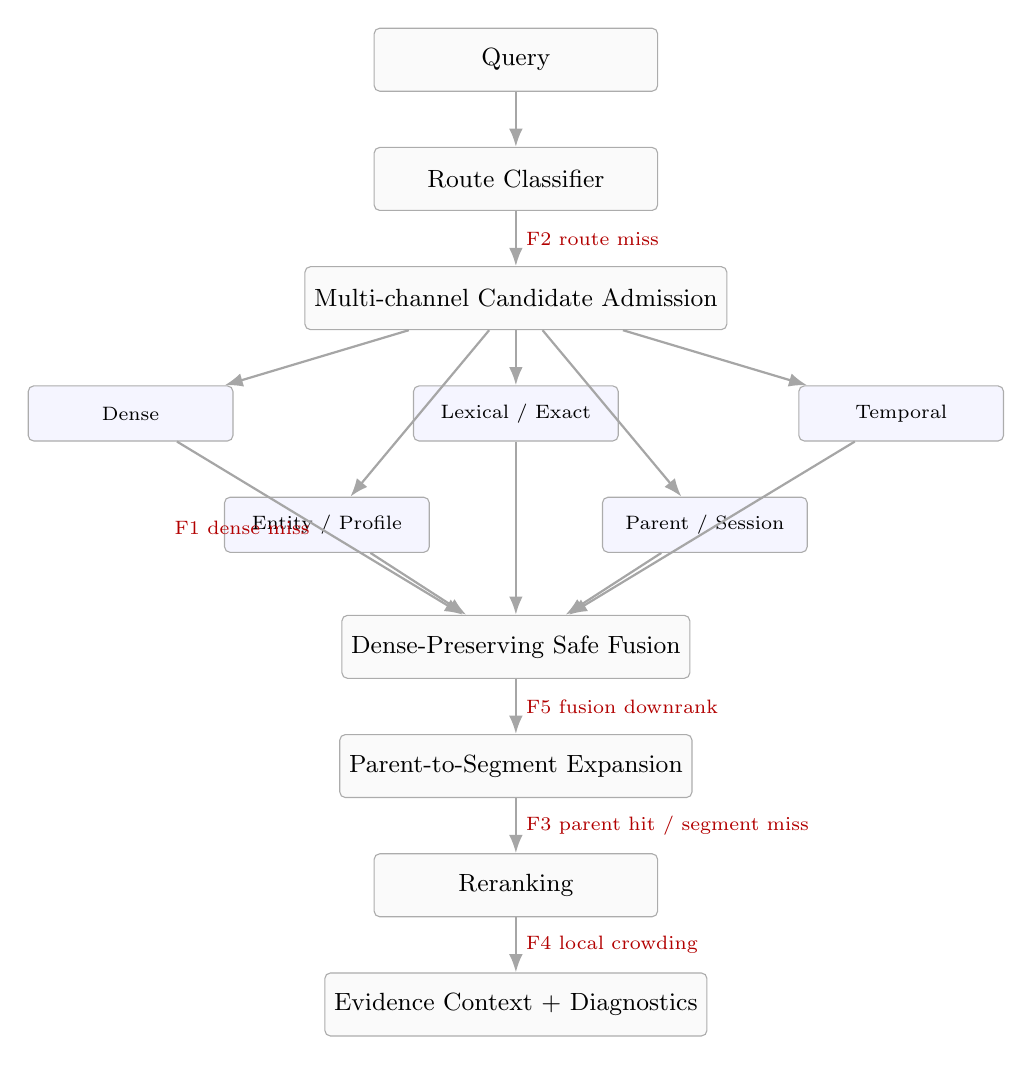
\begin{tikzpicture}[
  node distance=7mm and 9mm,
  box/.style={draw=gray!65, rounded corners=2pt, align=center, minimum width=36mm, minimum height=8mm, font=\small, fill=gray!4},
  chan/.style={draw=gray!65, rounded corners=2pt, align=center, minimum width=26mm, minimum height=7mm, font=\scriptsize, fill=blue!4},
  fail/.style={font=\scriptsize, text=red!70!black},
  arrow/.style={-Latex, thick, draw=gray!70}
]
\node[box] (query) {Query};
\node[box, below=of query] (route) {Route Classifier};
\node[box, below=of route] (admit) {Multi-channel Candidate Admission};
\node[chan, below left=of admit] (dense) {Dense};
\node[chan, below=of admit] (lex) {Lexical / Exact};
\node[chan, below right=of admit] (temporal) {Temporal};
\node[chan, below=of lex, xshift=-24mm] (entity) {Entity / Profile};
\node[chan, below=of lex, xshift=24mm] (parent) {Parent / Session};
\node[box, below=22mm of lex] (fusion) {Dense-Preserving Safe Fusion};
\node[box, below=of fusion] (segment) {Parent-to-Segment Expansion};
\node[box, below=of segment] (rerank) {Reranking};
\node[box, below=of rerank] (out) {Evidence Context + Diagnostics};

\draw[arrow] (query) -- (route);
\draw[arrow] (route) -- node[fail, right] {F2 route miss} (admit);
\draw[arrow] (admit) -- (dense);
\draw[arrow] (admit) -- (lex);
\draw[arrow] (admit) -- (temporal);
\draw[arrow] (admit) -- (entity);
\draw[arrow] (admit) -- (parent);
\draw[arrow] (dense) -- node[fail, left] {F1 dense miss} (fusion);
\draw[arrow] (lex) -- (fusion);
\draw[arrow] (temporal) -- (fusion);
\draw[arrow] (entity) -- (fusion);
\draw[arrow] (parent) -- (fusion);
\draw[arrow] (fusion) -- node[fail, right] {F5 fusion downrank} (segment);
\draw[arrow] (segment) -- node[fail, right] {F3 parent hit / segment miss} (rerank);
\draw[arrow] (rerank) -- node[fail, right] {F4 local crowding} (out);
\end{tikzpicture}

  \caption{Method flow and failure points. The figure shows route
  classification, multi-channel admission, dense-preserving fusion,
  parent-to-segment expansion, reranking, and diagnostic attribution.}
  \label{fig:pipeline}
\end{figure}

\begin{table*}[t]
  \centering
  \caption{Route-policy and budget metadata extracted from formal artifact
  metric files. Missing entries indicate that the formal artifact did not store
  the parameter, not that the value was zero.}
  \label{tab:route-policy}
  % Auto-generated by scripts/generate_paper_tables.py from formal artifact metric files.
\begin{tabular}{lllll}
\toprule
Parameter & LongMemEval & LoCoMo & KnowMe & CloneMem \\
\midrule
dense\_top\_k & not recorded & not recorded & not recorded & 200 \\
protected\_dense\_top\_m & not recorded & not recorded & not recorded & 100 \\
lexical\_top\_k & not recorded & not recorded & not recorded & 200 \\
temporal\_top\_k & not recorded & not recorded & not recorded & 90 \\
parent\_top\_k & not recorded & not recorded & not recorded & 50 \\
child\_segment\_cap & not recorded & not recorded & not recorded & 10 \\
final\_k & not recorded & not recorded & not recorded & 100 \\
fusion & not recorded & not recorded & not recorded & rrf \\
duplicate\_cap & not recorded & not recorded & not recorded & 1000 \\
route\_policy\_hash & not recorded & not recorded & not recorded & 9144917e6cd3c9e3eeef64bc709e02cbf2150b22b33c3a5f99cc05686c8bde51 \\
\bottomrule
\end{tabular}

\end{table*}

\section{Artifact-Backed Evaluation Protocol}

The formal protocol is a credibility layer, not the main contribution. It
checks that official rows are non-fallback, complete, registry-backed, and not
mixed with blocked or non-comparable artifacts. Historical runs are marked
\texttt{non\_comparable} when benchmark, run type, question scope, embedding,
fallback status, config hash, dataset version, or route policy differs.

\begin{table}[t]
  \centering
  \caption{Artifact validation coverage. Data source:
  \artifact{artifacts/formal\_protocol\_validation.json}.}
  \label{tab:artifact-validation}
  % Auto-generated by scripts/generate_paper_tables.py from artifacts/formal_protocol_validation.json.
\begin{tabular}{lrrrr}
\toprule
Evidence Section & Available & Blocked & Pending & Total \\
\midrule
ablations & 36 & 0 & 0 & 36 \\
baselines & 28 & 8 & 0 & 36 \\
efficiency & 7 & 0 & 0 & 7 \\
leave\_one\_benchmark\_out & 4 & 0 & 0 & 4 \\
statistics & 4 & 0 & 0 & 4 \\
\bottomrule
\end{tabular}

\end{table}

\section{Experiments}

\subsection{Benchmarks}

We evaluate LongMemEval, LoCoMo, KnowMe-Bench, and CloneMem. LongMemEval and
LoCoMo stress long dialogue and multi-session memory. KnowMe-Bench stresses
person understanding and lived-experience evidence. CloneMem stresses
non-conversational personal traces and AI-clone-style memory continuity
~\cite{wu2024longmemeval,maharana2024locomo,wu2026knowme,hu2026clonemem}.

\subsection{Baselines}

The main artifact table includes BM25, dense-only MiniLM, dense+BM25 RRF, and
\system{} full rows when available~\cite{robertson2009probabilistic,reimers2019sentencebert,cormack2009rrf}.
Blocked baselines such as unavailable cross-encoder/LLM rerankers and
dense-only BGE/E5 rows are not converted into improvement claims.

\subsection{Metrics}

We report admission recall at 100, final recall or fractional recall at 10,
NDCG at 10, elapsed seconds, and artifact status. For diagnostic sections, we
also report channel hit flags and failure categories.

\subsection{Implementation Details}

All official full rows use the sentence-transformers MiniLM backend without
local-hash fallback. CloneMem's protected top-3 lexical anchor gate is a
route-only policy with route-policy hash
\texttt{9144917e6cd3c9e3eeef64bc709e02cbf2150b22b33c3a5f99cc05686c8bde51}.
It is not a global CLI default.

\section{Results}

\subsection{Main Results}

\begin{table*}[t]
  \centering
  \caption{Formal full benchmark rows. Data source:
  \artifact{artifacts/formal\_protocol\_validation.json}. The admission-final
  gap is admission recall at 100 minus final recall at 10.}
  \label{tab:main-results}
  % Auto-generated by scripts/generate_paper_tables.py from artifacts/formal_protocol_validation.json.
\begin{tabular}{llrrrrrll}
\toprule
Benchmark & System & Q & Admission R@100 & Final R@10 & Gap & NDCG@10 & Run ID & Status \\
\midrule
longmemeval & DysonSpherain formal full & 500 & 1.0000 & 0.9778 & 0.0222 & 0.9259 & longmemeval-90e4c37dfb32 & passed \\
locomo & DysonSpherain formal full & 1986 & 1.0000 & 0.9070 & 0.0930 & 0.7533 & locomo-a19d4f7105c7 & passed \\
knowme & DysonSpherain formal full & 1010 & 0.7266 & 0.5972 & 0.1294 & 0.5051 & knowme-641f1fd83ba8 & passed \\
clonemem & DysonSpherain formal full & 2374 & 0.3442 & 0.0954 & 0.2488 & 0.0752 & clonemem-a40fef2bed79 & passed \\
\bottomrule
\end{tabular}

\end{table*}

\begin{table*}[t]
  \centering
  \caption{Available baseline rows. \system{} rows are taken from the formal
  full source-of-truth artifact; baseline rows come from artifact-backed
  baseline tables. Missing Admission R@100 means the baseline artifact did not
  record candidate-recall diagnostics, so those rows are not used to support
  admission-specific claims.}
  \label{tab:baseline-comparison}
  % Auto-generated by scripts/generate_paper_tables.py from paper/tables/main_results.tex.
% DysonSpherain rows are overwritten from artifacts/formal_protocol_validation.json to keep formal full metrics consistent.
% Missing baseline Admission R@100 means the source artifact did not record candidate-recall diagnostics.
\begin{tabular}{llrrrrll}
\toprule
Benchmark & Method & Admission R@100 & Recall@10 & NDCG@10 & Elapsed s & Comparability & Run ID \\
\midrule
clonemem & bm25 & -- & 0.0629 & 0.1022 & -- & available; admission may be unrecorded &  \\
clonemem & dense\_bm25\_rrf & -- & 0.0821 & 0.1265 & -- & available; admission may be unrecorded &  \\
clonemem & dense\_only\_minilm & -- & 0.0739 & 0.1094 & -- & available; admission may be unrecorded &  \\
clonemem & dysonspherain\_formal\_full & 0.3442 & 0.0954 & 0.0752 & 3429.8 & non\_comparable & clonemem-a40fef2bed79 \\
knowme & bm25 & -- & 0.4329 & 0.2862 & -- & available; admission may be unrecorded &  \\
knowme & dense\_bm25\_rrf & -- & 0.4168 & 0.3879 & -- & available; admission may be unrecorded &  \\
knowme & dense\_only\_minilm & -- & 0.5232 & 0.3656 & -- & available; admission may be unrecorded &  \\
knowme & dysonspherain\_formal\_full & 0.7266 & 0.5972 & 0.5051 & 1872.8 & non\_comparable & knowme-641f1fd83ba8 \\
locomo & bm25 & -- & 0.9059 & 0.7747 & -- & available; admission may be unrecorded &  \\
locomo & dense\_bm25\_rrf & -- & 0.9163 & 0.7170 & -- & available; admission may be unrecorded &  \\
locomo & dense\_only\_minilm & -- & 0.8340 & 0.6426 & -- & available; admission may be unrecorded &  \\
locomo & dysonspherain\_formal\_full & 1.0000 & 0.9070 & 0.7533 & 528.6 & non\_comparable & locomo-a19d4f7105c7 \\
longmemeval & bm25 & -- & 0.9620 & 0.8242 & -- & available; admission may be unrecorded &  \\
longmemeval & dense\_bm25\_rrf & -- & 0.9880 & 0.9089 & -- & available; admission may be unrecorded &  \\
longmemeval & dense\_only\_minilm & -- & 0.9880 & 0.8955 & -- & available; admission may be unrecorded &  \\
longmemeval & dysonspherain\_formal\_full & 1.0000 & 0.9778 & 0.9259 & 496.2 & non\_comparable & longmemeval-90e4c37dfb32 \\
\bottomrule
\end{tabular}

\end{table*}

\begin{figure}[t]
  \centering
  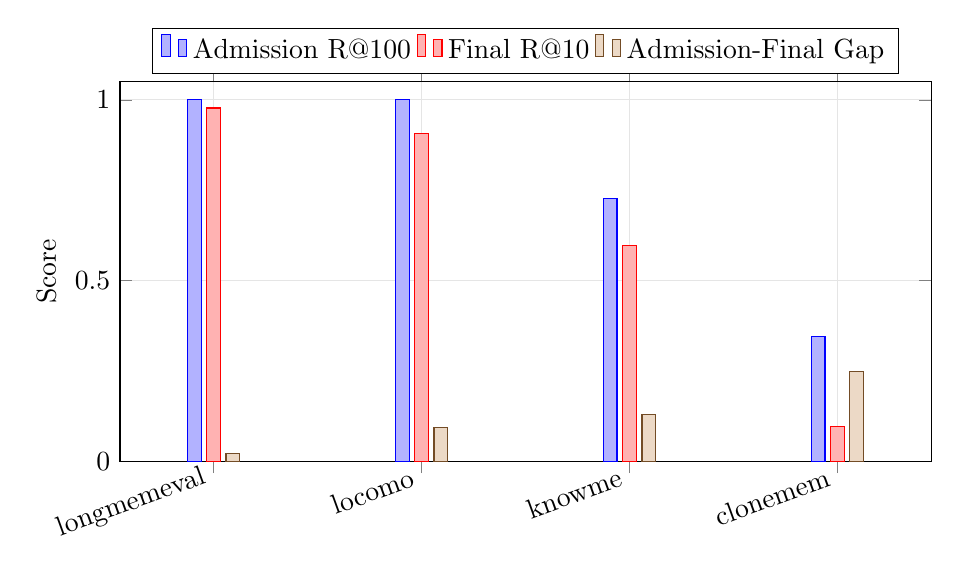
\begin{tikzpicture}
\begin{axis}[
  ybar, width=0.98\linewidth, height=6.4cm, ymin=0, ymax=1.05,
  ylabel={Score}, symbolic x coords={longmemeval,locomo,knowme,clonemem}, xtick=data, x tick label style={rotate=20, anchor=east},
  legend style={at={(0.5,1.02)}, anchor=south, legend columns=3},
  bar width=5pt, enlarge x limits=0.15, grid=major, grid style={draw=gray!20}]
\addplot coordinates {(longmemeval,1.0000) (locomo,1.0000) (knowme,0.7266) (clonemem,0.3442)};
\addplot coordinates {(longmemeval,0.9778) (locomo,0.9070) (knowme,0.5972) (clonemem,0.0954)};
\addplot coordinates {(longmemeval,0.0222) (locomo,0.0930) (knowme,0.1294) (clonemem,0.2488)};
\legend{Admission R@100,Final R@10,Admission-Final Gap}
\end{axis}
\end{tikzpicture}

  \caption{Admission-oriented benchmark view for formal full runs. The figure
  reports admission recall, final recall, and the admission-to-final gap rather
  than a generic benchmark score.}
  \label{fig:benchmark-comparison}
\end{figure}

LongMemEval and LoCoMo show strong first-stage coverage with admission recall
at 100 equal to 1.0. On these benchmarks, the remaining risk is less about
broad candidate recall and more about fusion, duplicate collapse, ordering, and
reranking. KnowMe-Bench exposes a different surface: admission recall is below
LongMemEval/LoCoMo, suggesting profile, preference, entity, and temporal-object
extraction remain incomplete. CloneMem remains a residual admission bottleneck
and is reported as a stress test rather than a success case.

\subsection{Ablations as Diagnostics}

\begin{table*}[t]
  \centering
\caption{Diagnostic ablation deltas generated from
  \artifact{paper/figures/data/ablation\_waterfall\_data.csv}. Deltas are
  relative to the ablation-family full row, not the formal full run. Positive
  values mean the ablated variant is higher on that metric.}
  \label{tab:ablations}
  % Auto-generated by scripts/generate_paper_tables.py from paper/figures/data/ablation_waterfall_data.csv.
% Deltas are against the ablation-family full_admission row, not against the formal full run.
\begin{tabular}{llrrrl}
\toprule
Benchmark & Removed Module & $\Delta$Admission R@100 & $\Delta$Final R@10 & $\Delta$NDCG@10 & Interpretation \\
\midrule
clonemem & -Route & 0.2308 & 0.0592 & 0.0497 & route policy sensitivity \\
clonemem & -Lexical & 0.2301 & 0.0754 & 0.0632 & lexical route can help anchors or add noise \\
clonemem & -Temporal & 0.2306 & 0.0578 & 0.0535 & temporal route is surface-dependent \\
clonemem & -Parent2Seg & 0.2306 & 0.0355 & 0.0306 & parent-to-segment selection risk \\
clonemem & -SafeFusion & 0.2432 & 0.0703 & 0.0505 & dense protection tradeoff \\
knowme & -Route & 0.0005 & -0.0010 & -0.0013 & route policy sensitivity \\
knowme & -Lexical & -0.0074 & 0.0104 & -0.0039 & lexical route can help anchors or add noise \\
knowme & -Temporal & 0.0008 & -0.0037 & -0.0025 & temporal route is surface-dependent \\
knowme & -Parent2Seg & -0.0037 & -0.0011 & -0.0039 & parent-to-segment selection risk \\
knowme & -SafeFusion & 0.0054 & -0.0133 & -0.0202 & dense protection tradeoff \\
locomo & -Route & 0.0000 & 0.0000 & 0.0000 & route policy sensitivity \\
locomo & -Lexical & 0.0000 & -0.0543 & -0.0885 & lexical route can help anchors or add noise \\
locomo & -Temporal & 0.0000 & -0.0005 & -0.0008 & temporal route is surface-dependent \\
locomo & -Parent2Seg & 0.0000 & 0.0015 & 0.0006 & parent-to-segment selection risk \\
locomo & -SafeFusion & 0.0000 & 0.0077 & 0.0098 & dense protection tradeoff \\
longmemeval & -Route & 0.0000 & 0.0000 & 0.0000 & route policy sensitivity \\
longmemeval & -Lexical & 0.0000 & -0.0046 & -0.0219 & lexical route can help anchors or add noise \\
longmemeval & -Temporal & 0.0000 & 0.0037 & -0.0014 & temporal route is surface-dependent \\
longmemeval & -Parent2Seg & 0.0000 & 0.0000 & 0.0000 & parent-to-segment selection risk \\
longmemeval & -SafeFusion & 0.0000 & 0.0047 & 0.0039 & dense protection tradeoff \\
\bottomrule
\end{tabular}

\end{table*}

The ablation table should be read as diagnostic evidence, not as proof that
every module is monotonically beneficial. Several ablated variants outperform
the ablation-family full run on specific benchmarks. This is a finding rather
than an inconsistency: admission mechanisms are surface-dependent. Lexical and
temporal routes can recover anchors on one memory surface while adding noisy
candidates on another; safe fusion can protect dense anchors while suppressing
some sparse signals; parent expansion can repair parent-hit segment-miss cases
while over-expanding local clusters. \system{} is therefore a diagnostic and
guarded route-conditioned framework, not a universal additive recipe.

\subsection{Failure Analysis}

CloneMem exposes the clearest residual failure. Candidate recall at 100 remains
low and final recall/NDCG are also low. This points to first-stage admission
over non-conversational, longitudinal, person-state traces rather than a pure
final-reranking issue. The next mechanism frontier is a non-conversational
trace route, stronger profile-state extraction, and temporal object extraction.

KnowMe-Bench also separates first-stage and final ordering failures. Its
admission recall is lower than LongMemEval/LoCoMo, so the likely bottleneck is
profile and preference evidence admission before final reranking.

\begin{figure}[t]
  \centering
  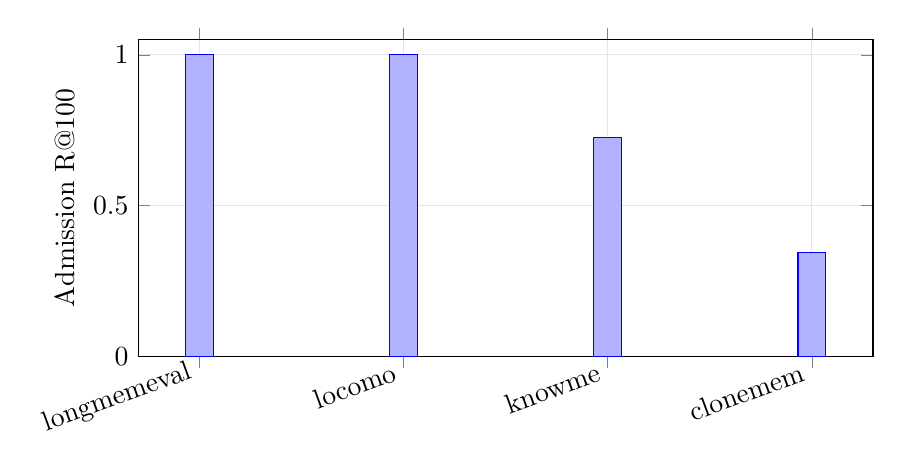
\begin{tikzpicture}
\begin{axis}[ybar,width=0.9\linewidth,height=5.6cm,ymin=0,ymax=1.05,ylabel={Admission R@100},symbolic x coords={longmemeval,locomo,knowme,clonemem},xtick=data,x tick label style={rotate=20,anchor=east},grid=major,grid style={draw=gray!20}]
\addplot coordinates {(longmemeval,1.0000) (locomo,1.0000) (knowme,0.7266) (clonemem,0.3442)};
\end{axis}
\end{tikzpicture}

  \caption{Admission recall by full formal benchmark. CloneMem and KnowMe show
  residual admission bottlenecks relative to LongMemEval and LoCoMo.}
  \label{fig:failure-breakdown}
\end{figure}

\subsection{Efficiency Analysis}

\begin{figure}[t]
  \centering
  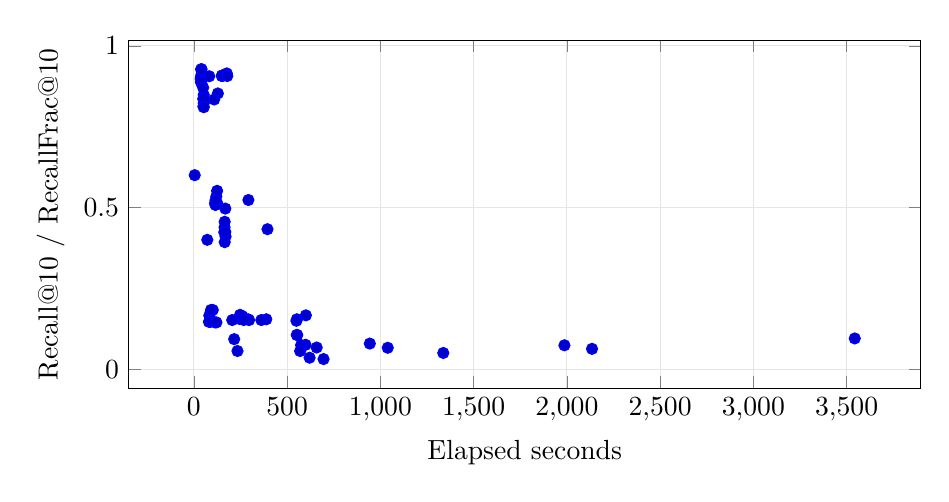
\begin{tikzpicture}
\begin{axis}[width=0.96\linewidth,height=6cm,xlabel={Elapsed seconds},ylabel={Recall@10 / RecallFrac@10},grid=major,grid style={draw=gray!20}]
\addplot+[only marks, mark=*] coordinates {
(4.747,0.6000)
(599.089,0.0754)
(620.677,0.0355)
(234.051,0.0562)
(695.508,0.0313)
(575.123,0.0746)
(2134.924,0.0629)
(291.329,0.1543)
(260.017,0.1640)
(267.204,0.1555)
(600.680,0.1665)
(247.767,0.1680)
(3543.535,0.0951)
(388.478,0.1543)
(552.575,0.1543)
(550.036,0.1497)
(244.605,0.1555)
(296.195,0.1518)
(101.700,0.1831)
(90.175,0.1464)
(113.862,0.1447)
(205.804,0.1520)
(151.371,0.9070)
(152.359,0.9070)
(128.776,0.8527)
(152.195,0.9084)
(151.500,0.9070)
(150.376,0.9070)
(176.728,0.9147)
(179.163,0.9065)
(165.632,0.3929)
(164.297,0.4248)
(168.850,0.4966)
(164.626,0.4389)
(170.290,0.4101)
(164.217,0.4223)
(168.683,0.4246)
(165.360,0.4558)
(394.855,0.4329)
(83.001,0.1660)
(72.213,0.4000)
(40.654,0.9098)
(41.623,0.9278)
(38.329,0.8872)
(41.556,0.9059)
(36.906,0.8978)
(37.954,0.9025)
(38.830,0.8905)
(38.758,0.9272)
(82.701,0.9059)
(551.950,0.1060)
(1039.622,0.0662)
(569.883,0.0561)
(216.392,0.0929)
(1337.444,0.0502)
(658.663,0.0670)
(554.585,0.1057)
(943.557,0.0792)
(1986.982,0.0739)
(91.938,0.1831)
(80.875,0.1464)
(121.081,0.1447)
(267.687,0.1520)
(361.833,0.1520)
(126.492,0.5115)
(120.493,0.5342)
(124.794,0.5515)
(113.743,0.5131)
(115.934,0.5078)
(116.017,0.5223)
(292.540,0.5232)
(52.631,0.8362)
(53.201,0.8229)
(50.531,0.8358)
(52.982,0.8485)
(51.197,0.8127)
(54.110,0.8364)
(53.382,0.8102)
(50.043,0.8708)
(109.145,0.8340)
};
\end{axis}
\end{tikzpicture}

  \caption{Efficiency-quality surface from available artifacts. Points mix
  available diagnostic and formal records, so the figure is descriptive rather
  than a matched improvement claim.}
  \label{fig:efficiency-pareto}
\end{figure}

Phase 13 provides seven matched budget artifacts for candidate and rerank
budgets. Where matched quality metrics are unavailable for every budget, the
paper keeps the efficiency plot descriptive and avoids inventing a Pareto gain.

\begin{table}[t]
  \centering
  \caption{CloneMem full-run efficiency update. The April 30 run is included as
  runtime evidence only: it uses the official embedding/vector path and covers
  the full CloneMem question set, but it does not change the paper's quality
  conclusion because candidate admission remains low.}
  \label{tab:clonemem-efficiency}
  % Auto-generated by scripts/generate_paper_tables.py from formal validation and the 2026-04-30 CloneMem efficiency artifact.
\begin{tabular}{lrrrrrr}
\toprule
Run & Q & Wall s & Speedup & Admission R@100 & Final R@10 & Final NDCG@10 \\
\midrule
Formal full & 2374 & 3429.8 & -- & 0.3442 & 0.0954 & 0.0752 \\
Apr. 30 efficiency & 2374 & 1789.9 & 3.34 & 0.3436 & 0.0950 & 0.0749 \\
\bottomrule
\end{tabular}

\vspace{2pt}

\parbox{0.96\linewidth}{\footnotesize The efficiency run is official-embedding and Chroma-backed, but it is used as runtime evidence; quality remains a warning because CloneMem candidate recall is still low. Serial shard time sums to 5983.4 seconds.}

\end{table}

The April 30 CloneMem efficiency run reduces full-run wall-clock time from the formal source-of-truth row's 3429.8 seconds to 1789.9 seconds on the same 2374 questions, with a 3.34$\times$ shard-level speedup estimate. This is an engineering result, not a retrieval-quality result: candidate recall at 100 is 0.3436 and final recall at 10 is 0.0950, matching the existing CloneMem bottleneck profile. The manuscript therefore updates the runtime claim while preserving the conclusion that CloneMem remains unsolved.


\section{Case Studies}

\begin{table}[t]
  \centering
  \caption{Diagnostic case-study examples extracted from JSONL artifacts.}
  \label{tab:case-studies}
  % Auto-generated by scripts/generate_case_studies.py from reports/diagnostics/*.jsonl.
\begin{tabular}{lrrrrrl}
\toprule
Case & Dense Rank & Fused Rank & Parent Rank & Segment Rank & Final Rank & Fixed By \\
\midrule
1. Temporal anchoring drift & 21 & 21 & -- & 21 & 55 & not fixed \\
2. Parent-hit segment miss & 136 & -- & -- & -- & -- & not fixed \\
3. Reranker dropped gold & 1 & 1 & -- & 1 & 12 & not fixed \\
4. KnowMe segment admission failure & -- & -- & -- & -- & -- & not fixed \\
\bottomrule
\end{tabular}

\end{table}

% Auto-generated by scripts/generate_case_studies.py.

\subsection{Diagnostic Case Studies}

The examples below are extracted from diagnostic JSONL artifacts and redacted/truncated for paper use. They illustrate failure attribution rather than new benchmark claims.

\paragraph{Case 1: Temporal anchoring drift.}

Benchmark: \texttt{clonemem}. Failure type: \texttt{temporal\_miss}. Admission R@100 for the query is 0.5; final R@10 is 0.0. Dense rank: 21; fused rank: 21; final rank: 55. Gold-hitting channels: dense\_semantic, entity\_aware, exact\_phrase, lexical\_sparse. Query excerpt: ``[redacted]15[redacted]25[redacted]7[redacted]''

\paragraph{Case 2: Parent-hit segment miss.}

Benchmark: \texttt{clonemem}. Failure type: \texttt{parent\_hit\_segment\_miss}. Admission R@100 for the query is 0.0; final R@10 is 0.0. Dense rank: 136; fused rank: --; final rank: --. Gold-hitting channels: dense\_semantic, entity\_aware, lexical\_sparse. Query excerpt: ``Old Chen, when you decided to delete that "Family Health Management Spreadsheet" back in early September, did you ever stop to think how things between you and Meifang...''

\paragraph{Case 3: Reranker dropped gold.}

Benchmark: \texttt{clonemem}. Failure type: \texttt{reranker\_dropped\_gold}. Admission R@100 for the query is 0.8; final R@10 is 0.0. Dense rank: 1; fused rank: 1; final rank: 12. Gold-hitting channels: dense\_semantic, entity\_aware, exact\_phrase, lexical\_sparse. Query excerpt: ``Old Chen, I remember you mentioning that "stability" is your guiding principle, but over the past month or so, I feel like you[redacted]ve changed quite a bit. First,...''

\paragraph{Case 4: KnowMe segment admission failure.}

Benchmark: \texttt{knowme}. Failure type: \texttt{parent\_hit\_segment\_miss}. Admission R@100 for the query is 0.0; final R@10 is 0.0. Dense rank: --; fused rank: --; final rank: --. Gold-hitting channels: lexical\_sparse, temporal\_neighbor. Query excerpt: ``What are the names of the two rats who shot at Karl Larsdal and the narrator in the garbage dump?''


\section{Related Work}

\paragraph{Long-horizon memory benchmarks.}
LongMemEval and LoCoMo emphasize long dialogue and multi-session memory.
KnowMe-Bench emphasizes person understanding and lived-experience evidence.
CloneMem emphasizes non-conversational personal traces and AI-clone-style
continuity~\cite{wu2024longmemeval,maharana2024locomo,wu2026knowme,hu2026clonemem}.
Other agent-memory benchmarks cover adjacent surfaces including tool-use,
life-assistant memory, and episodic or semantic memory evaluation. \system{}
differs by focusing on the admission layer before generation.

\paragraph{Agent memory systems.}
Systems such as Mem0, MemGPT/Letta, LangMem, MemoryBank, Generative Agents,
Reflexion, and MemAgent study memory writing, updating, retrieval, reflection,
and agent behavior~\cite{mem02024,packer2023memgpt,langmem2025,zhong2023memorybank,park2023generativeagents,shinn2023reflexion}.
This paper is narrower: it treats candidate admission as a measurable
retrieval failure layer and reports diagnostics that distinguish admission,
fusion, parent-to-segment, and reranking failures.

\paragraph{Retrieval and reranking.}
Dense retrieval, BM25, hybrid retrieval, reciprocal rank fusion, cross-encoder
reranking, parent-child retrieval, and multi-stage retrieval are standard tools
for document retrieval and RAG~\cite{robertson2009probabilistic,karpukhin2020dense,cormack2009rrf,nogueira2019passage,lewis2020rag}.
\system{} is not simply hybrid retrieval: it uses route-conditioned channel
selection, dense-preserving fusion, bounded parent-to-segment expansion, and
diagnostic attribution for long-horizon memory queries.

\paragraph{Personalization and temporal memory.}
Personal memory systems must reason over temporal context, entity-centric
state, preferences, profile changes, and forgetting. These requirements make
privacy and provenance central rather than peripheral.

\section{Limitations}

This paper does not claim universal state of the art. Historical runs marked
\texttt{non\_comparable} are not used for improvement claims. CloneMem remains
a residual admission bottleneck. Ablations are not monotonic across benchmarks,
which means route-policy selection remains a research problem. Baseline
admission metrics still require full comparable reruns when candidate-recall
diagnostics were not stored. Route policies carry benchmark-specific tuning
risk and should not be treated as global defaults. The method optimizes
retrieval and admission; it does not directly solve generation hallucination.
The validation protocol blocks local embedding fallback from entering formal
tables. Finally, benchmark gold granularity may not always match the system's
memory segmentation, making parent-to-segment selection a continuing source of
error.

\section{Ethics and Privacy Considerations}

Long-term personal memory can contain sensitive information about identity,
preferences, health, emotions, routines, relationships, and behavior patterns.
Systems should not infer sensitive attributes by default. Practical deployments
need deletion, forgetting, redaction, provenance tracking, and retrieval traces.
AI-clone scenarios can amplify privacy and identity-simulation risks, so
benchmark performance should not be interpreted as sufficient proof of real
user-modeling safety. Future CLI, email, calendar, or code-agent memory
integrations should be opt-in, local-first where possible, and governed by
user-controlled retention policies.

\section{Conclusion}

\system{} reframes long-horizon agent memory retrieval around candidate
admission failures. The method combines route-conditioned admission,
dense-preserving safe fusion, and parent-to-segment anchoring, while the
artifact protocol prevents fallback, blocked, and non-comparable evidence from
becoming inflated claims. The current results show strong admission on
LongMemEval and LoCoMo, expose profile and trace bottlenecks on KnowMe and
CloneMem, and define a concrete next frontier for non-conversational personal
memory retrieval.

\appendix

\section{Artifact Schema and Validation Protocol}

Formal evidence is validated through artifact JSON, registry metadata,
fallback flags, dataset and config hashes, route-policy hashes, and explicit
blocked/non-comparable statuses. The summary table in
Table~\ref{tab:artifact-validation} is generated from
\artifact{artifacts/formal\_protocol\_validation.json}.

\section{Full Benchmark Tables}

The full paper-facing baseline table is generated by
\artifact{scripts/generate\_paper\_tables.py}. Blocked unavailable-model rows
remain in artifact reports but are excluded from main improvement claims.

\section{Full Ablation Tables}

Table~\ref{tab:ablations} is generated from the ablation CSV and should be
interpreted together with benchmark-specific comparability notes.

\section{Failure Taxonomy}

\begin{table}[h]
  \centering
  \caption{Failure taxonomy artifact rows.}
  % Auto-generated by scripts/generate_paper_tables.py from paper/figures/data/failure_bucket_delta.csv.
\begin{tabular}{llr}
\toprule
Benchmark & Ablation & Artifact Rows \\
\midrule
clonemem & full\_admission & 1 \\
clonemem & no\_benchmark\_route\_tuning & 1 \\
clonemem & no\_inhibition & 1 \\
clonemem & no\_lexical\_probe & 1 \\
clonemem & no\_parent\_to\_segment\_selector & 1 \\
clonemem & no\_rerank\_guard & 1 \\
clonemem & no\_route\_conditioned\_admission & 1 \\
clonemem & no\_safe\_fusion & 1 \\
clonemem & no\_temporal\_routing & 1 \\
knowme & full\_admission & 1 \\
knowme & no\_benchmark\_route\_tuning & 1 \\
knowme & no\_inhibition & 1 \\
knowme & no\_lexical\_probe & 1 \\
knowme & no\_parent\_to\_segment\_selector & 1 \\
knowme & no\_rerank\_guard & 1 \\
knowme & no\_route\_conditioned\_admission & 1 \\
knowme & no\_safe\_fusion & 1 \\
knowme & no\_temporal\_routing & 1 \\
locomo & full\_admission & 1 \\
locomo & no\_benchmark\_route\_tuning & 1 \\
locomo & no\_inhibition & 1 \\
locomo & no\_lexical\_probe & 1 \\
locomo & no\_parent\_to\_segment\_selector & 1 \\
locomo & no\_rerank\_guard & 1 \\
locomo & no\_route\_conditioned\_admission & 1 \\
locomo & no\_safe\_fusion & 1 \\
locomo & no\_temporal\_routing & 1 \\
longmemeval & full\_admission & 1 \\
longmemeval & no\_benchmark\_route\_tuning & 1 \\
longmemeval & no\_inhibition & 1 \\
longmemeval & no\_lexical\_probe & 1 \\
longmemeval & no\_parent\_to\_segment\_selector & 1 \\
longmemeval & no\_rerank\_guard & 1 \\
longmemeval & no\_route\_conditioned\_admission & 1 \\
longmemeval & no\_safe\_fusion & 1 \\
longmemeval & no\_temporal\_routing & 1 \\
\bottomrule
\end{tabular}

\end{table}

\section{Additional Case Studies}

Additional diagnostic examples can be regenerated with
\artifact{scripts/generate\_case\_studies.py}.

\section{Hyperparameters and Compute}

Official full rows report elapsed seconds in Table~\ref{tab:main-results}.
Route budgets and config hashes are tracked in the benchmark artifacts and
registry. No cross-encoder or unavailable BGE/E5 rows are promoted into formal
results.

\section{NeurIPS Checklist}

The current draft includes limitations, ethics, reproducibility notes,
artifact-backed tables, and explicit blocked/non-comparable status handling.

\bibliographystyle{plain}
\bibliography{references}

\end{document}
